\section{Basics of Information Theory}

When we talk about \textit{information}, we often use the term in qualitative sense. We say things like 
\textit{This is valuable information} or 
\textit{We have a lack of information}. We can also make statements about some information being more helpful than other. For a long time, however,
people have been unable to quantify information. The person who succeeded in this endeavour was \href{https://en.wikipedia.org/wiki/Claude_Shannon}{Claude E. Shannon}
who with his famous 1948 article \textit{A Mathematical Theory of Communication} single-handedly created a new discipline: Information Theory! He also revolutionised
digital communication and can be seen as one of the main contributors to our modern communication systems like the telephone, the internet etc. 

The beauty about information theory is that it is based on probability theory and many results from probability theory seamlessly carry over to information theory.
In this chapter, we are going to discuss the bare basics of information theory. These basics are often enough to understand many information theoretic arguments
that researchers make in fields like computer science, psychology and linguistics.

Shannon's idea of information is as simple as it is compelling. Intuitively, if we are observing a realisation of a random variable, this realisation is surprising
if it is unlikely to occur according to the distribution of that random variable. However, if the probability for the realisation is very low, than on average it
does not occur very often, meaning that if we sample from the RV repeatedly, we are not surprised very often. We are not surprised when the probability
mass of the distribution is concentrated on only a small subset of its support. 

On the other hand, we quite often are surprised,
if we cannot predict what the outcome of our next draw from the RV might be. We are surprised when the distribution over values of the RV is (close to) uniform. Thus,
we are going to be most surprised on average if we are observing realisations of a uniformly distributed RV.

Shannon's idea was that observing RVs that cause a lot of surprises is informative because we cannot predict the outcomes and with each new outcome we have effectively
learned something  (namely that the $ i^{th} $ outcome took on the value that it did). Observing RVs with very concentrated distributions is not very informative
under this conception because by just choosing the most probable outcome we can correctly predict most actually observed outcomes. Obviously, if I manage to predict
an outcome beforehand, it's occurrence is not teaching me anything.

The goal of Shannon was to find a function that captures this intuitive idea. He eventually found it and showed that it is the only function to have properties
that encompass the intuition. This function is called the \textbf{entropy} of a RV and it is simply the expected \textbf{surprisal} value.

\begin{Definition}[Surprisal]
The surprisal (value) of an outcome $ x \in \supp(X) $ of some RV $ X $ is defined as $ -\log_{2}(P(X=x))$.
\end{Definition} 

Notice that we are using the logarithm of base 2 here. This is because surprisal and entropy are standardly measured in bits. Intuitively, the surprisal measures
how many bits one needs to encode an observed outcome given that one knows the distribution underlying that outcome. The entropy measures how many bits one
will need on average to encode an outcome that is generated by the distribution $ P_{X} $.

\begin{Definition}[Entropy]
The entropy $H(P_X)$ of a RV $ X $ with distribution $P_X$ is defined as 
$$H(P_X) := \E[-\log_{2}(P(X=x))] = - \!\! \sum_{x \in \supp(X)} P(X=x) \log_2(P(X=x)) \, .$$ 
For the ease of notation, we often write $H(X)$ instead of $H(P_X)$.
\end{Definition}

Figure~\ref{fig:binaryEntropy} shows the entropy of the Bernoulli distribution as a function of the
parameter $ \theta $. The entropy function of the Bernoulli is often called the \textbf{binary entropy}.
It measures the information of a binary decision, like a coin flip or an answer to a yes/no-question.
The entropy of the Bernoulli is 1 bit when the distribution is uniform, i.e.\ when both choices are equally 
probable. 

\begin{figure}
\center
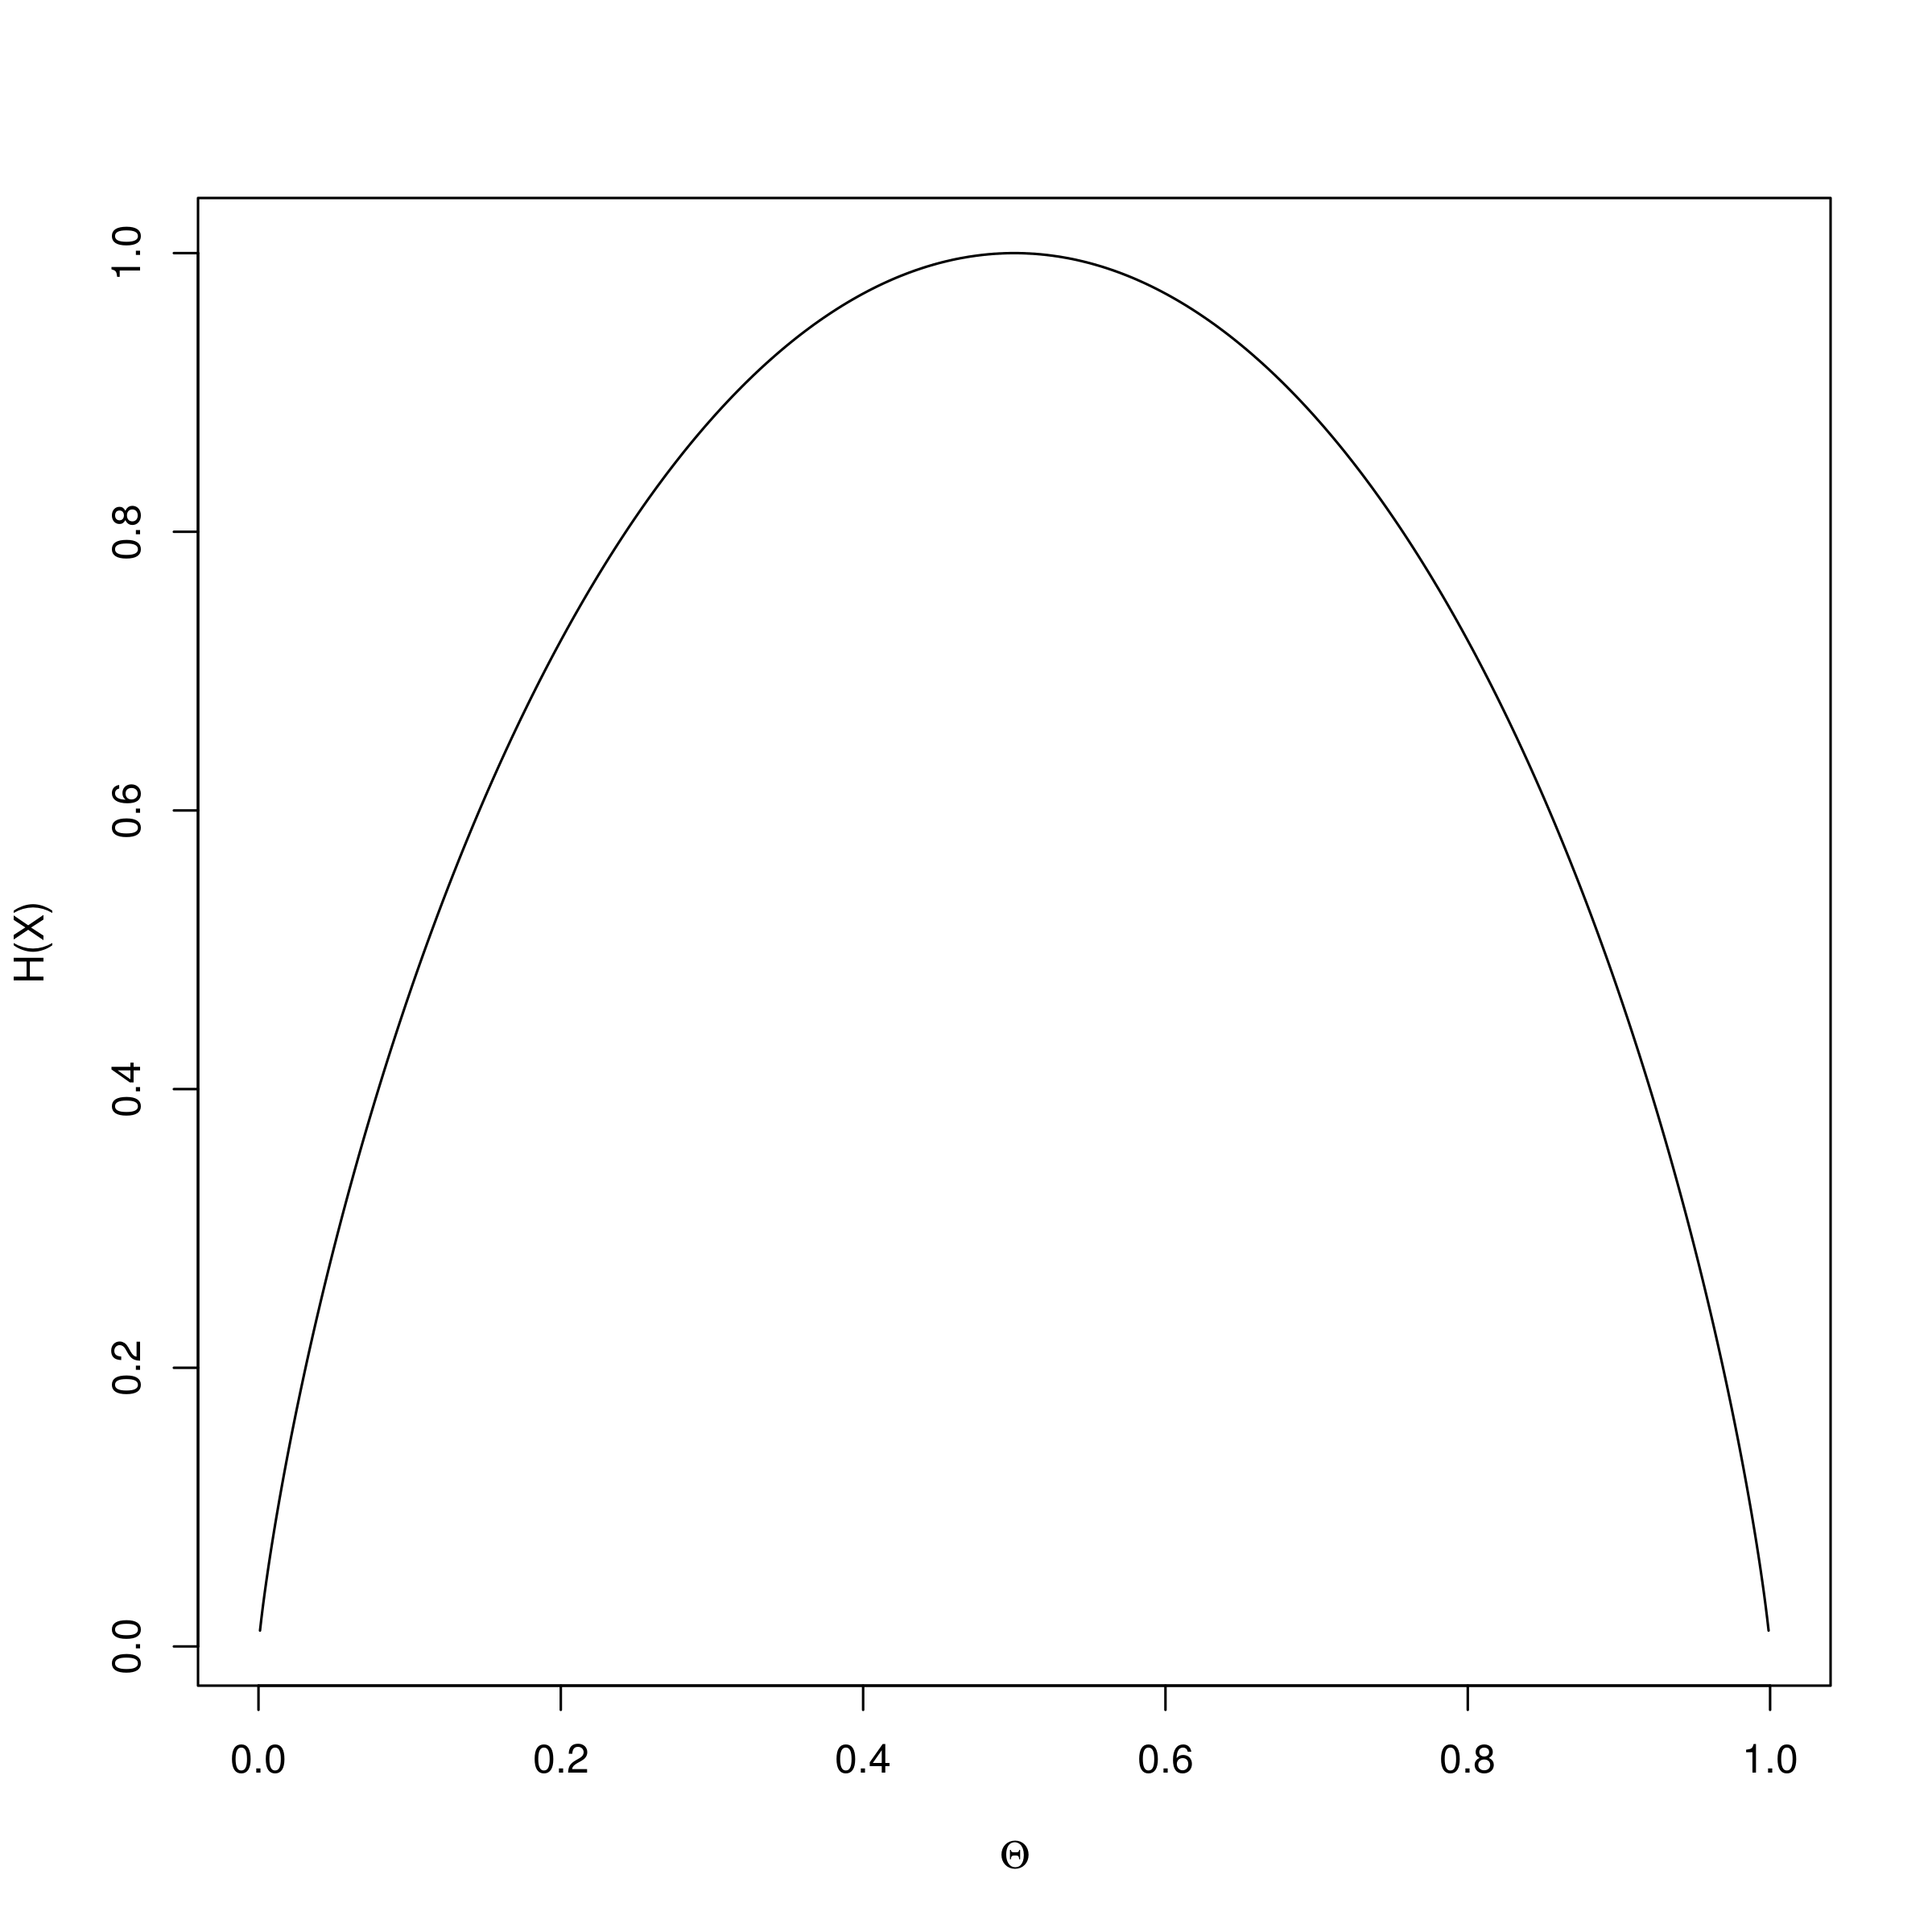
\includegraphics[scale=0.4]{binaryEntropy.png}
\caption{Binary entropy function.}
\label{fig:binaryEntropy}
\end{figure}

From the plot is it also easy to see that entropy is never negative. It holds in general that entropy is non-negative,
because entropy is defined as expectation of surprisal and surprisal is the negative logarithm of probabilities. 
Because $ \log(x) \leq 0 $ for $ x \in (0,1] $, it is clear that $ -\log(x) \geq 0 $ for $ x $ in the same
interval. Notice that from here on we drop the subscript and by convention let $ \log = \log_{2} $.

A standard interpretation of the entropy is that it quantifies uncertainty. As we have pointed out
before, a uniform distribution means that you are most uncertain and
indeed the uniform distribution maximizes the entropy. However, the more choices you have to pick from, the more uncertain you are going to be. 
The entropy function also captures this intuition. Notice that if a discrete distribution is uniform,
all probabilities are $ \frac{1}{|\supp(X)|} $. Clearly, as we increase $ |\supp(X)| $, we decrease the
probabilities. By decreasing the probabilities, we increase their negative logarithms, and hence their
surprisal. Let us make this intuition more formal.

\begin{Theorem}
A discrete RV $ X $ with uniform distribution and support of size $ n $ has entropy
$ H(X) = \log(n) $.
\end{Theorem}

\paragraph{Proof:}
\begin{align}
H(X) &= \underset{x \in \supp(X)}{\sum}-\log(P(X=x))P(X=x) \\
&= \underset{x \in \supp(X)}{\sum}\log(n)P(X=x) = \log(n) \, . ~~~~\square
\end{align}

\begin{Exercise}
You are trying to learn chess and you start by studying where chess grandmasters move their king when it
is positioned in one of the middle fields of the board. The king can move to any of the adjoining 8 fields. Since
you do not know a thing about chess yet, you assume that each move is equally probable. In this situation,
what is the entropy of moving the king?
\end{Exercise}

At the outset of this section we promised you that you could easily transfer results from probability 
theory to information theory. We will not be able to show any kind of linearity for entropy because it contains
log-terms and the logarithm is not linear. We can however find alternative expressions for joint entropy (where 
the joint entropy is simply the entropy of a joint RV). Before we do so, let us also define the notion of 
conditional entropy. We have seen in Section~\ref{sec:jointconditionaldistributions} that $P_{X|Y=y}$ is a valid probability distribution for any $y \in \supp(Y)$ such that $P(Y=y)>0$. Hence, we can also define its conditional entropy.

\begin{Definition}[Conditional Entropy]
For two jointly distributed RVs $ X,Y $ and $y \in \supp(Y)$ such that $P(Y=y)>0$, the conditional entropy of $ X $ given that $ Y=y $ is defined as
\begin{align*}
H(X|Y=y) &:= \E_X[-\log_{2}(P(X=x|Y=y))] \\
&= - \!\! \sum_{x \in \supp(X)} P(X=x|Y=y) \log_2(P(X=x|Y=y))\, . 
\end{align*}
The conditional entropy of $X$ given $Y$ is defined as
$$ H(X|Y) := \E_Y[ H(X|Y) ] = \sum_{y \in \supp(Y)} P(Y=y) H(X|Y=y) \, .$$
\end{Definition}

With this definition at hand we show that the joint entropy decomposes according to the
chain rule.

\begin{align*}
H(X,Y) &= \underset{\substack{x \in \supp(X)\\y \in \supp(Y)}}{\sum} -\log(P(X=x,Y=y)) \times P(X=x, Y=y) \\
\begin{split}
&= \underset{\substack{x \in \supp(X)\\ y \in \supp(Y)}}{\sum} -\log(P(X=x| Y=y)) \times P(X=x,Y=y) \\ 
&\qquad - \underset{y \in \supp(Y)}{\sum}\log(P(Y=y)) \times \sum_{x \in \supp(X)} P(X=x,Y=y) 
\end{split} \\
\begin{split}
&=\sum_{y \in \supp(Y)} P(Y=y) \times \sum_{x \in \supp(X)} -\log(P(X=x| Y=y)) \times P(X=x|Y=y) \\ &\qquad - \underset{y \in \supp(Y)}{\sum}\log(P(Y=y)) \times P(Y=y)
\end{split} \\
&= H(X|Y) + H(Y)
\end{align*}

\begin{Exercise}
Prove that $ H(X,Y|Z) = H(X|Z) + H(Y|Z) $ if $ X \bot Y|Z $.
\end{Exercise}

Now that we have seen some information-theoretic concepts, you may be happy to hear that there is an information-theoretic interpretation
of EM. This interpretation helps us to get a better intuition for the algorithm. To formulate that interpretation we need
one more concept, however.

\begin{Definition}[Relative Entropy]
The relative entropy of RVs \\ $ X,Y $ with distributions $P_X, P_Y$ and $\supp(X) \subseteq \supp(Y) $ is defined as
$$ D(P_X||P_Y) := \sum_{x \in \supp(X)} P(X=x) \log \frac{P(X=x)}{P(Y=x)} \ . $$
If $ P(X=y) = 0 $ for any $ y \in \supp(Y) $ we define $ D(P_X||P_Y) = \infty $. As with entropy, we often abbreviate $D(P_X||P_Y)$ with  $D(X||Y)$.
\end{Definition}

The relative entropy is commonly known as \textbf{Kullback-Leibler (KL)} divergence. It measures the entropy of $ X $ as scaled to $ Y $. Intuitively,
it gives a measure of how ``far away'' $ P_{X} $ is from $ P_{Y} $. To
understand ``far away'', recall that entropy is a measure of
uncertainty. 
% The
% relative entropy measure the uncertainty that you have about $ P_{X} $ if you know $ P_{Y} $\chris{hard to see why at this point}.
This uncertainty is low if both distributions place most
of their mass on the same outcomes. Since $ \log(1) = 0 $ the relative entropy is 0 if $ P_{X} = P_{Y} $.

It is worthwhile to point out the difference between relative and conditional entropy. Conditional entropy is the average entropy of $ X $ given that you
know what value $ Y $ takes on. In the case of relative entropy you do not know the value of $ Y $, only its distribution.

\begin{Exercise}
Show that $ D(X,Y||Y) = H(X|Y) $. Furthermore show that $ D(X,Y||Y) = H(X) $ if $ X\bot Y $.
\end{Exercise}


\section{An Information-Theoretic View on EM}

Let us start by remembering why we need EM. We have a model that defines a joint distribution
over observed ($ x $) and latent data ($ z $). Such a model generally looks as follows:
\begin{equation}
P(X=x, Z=z | \Theta = \theta) = P(X=x|Z=z, \Theta=\theta) P(Z=z|\Theta = \theta)
\end{equation}
where we have chosen a factorization that provides a separate term for a distribution over only the
latent data.

Recall that the goal of the EM algorithm is to iteratively increase the likelihood through consecutive
updates of parameter estimates. These updates are achieved through maximum likelihood estimation based
on expected sufficient statistics. We are now going to show that a) EM computes a lower bound on the
marginal log-likelihood of the data in each iteration and b) that this lower bound becomes tight when the
expected sufficient statistics are taken with respect to the model posterior. The latter implies that
EM performs the optimal update in each iteration.

Let us start by expanding the data log-likelihood and then lower-bounding it.
\begin{align}
&\log(P(X=x|\Theta=\theta)) = \sum_{y} \log(P(X=x, Y=y| \Theta = \theta))  \\
&= \sum_{y} \log\left(Q(Y=y|\Phi=\phi)\frac{P(X=x, Y=y| \Theta = \theta)}{Q(Y=y|\Phi=\phi)}\right) \\
&\geq \sum_{y} Q(Y=y|\Phi=\phi) \log\left(\frac{P(X=x, Y=y| \Theta = \theta)}{Q(Y=y|\Phi=\phi)}\right)
\label{eq:ELBO1}
\end{align}
Here, we have used \href{https://en.wikipedia.org/wiki/Jensen\%27s_inequality}{Jensen's Inequality} to
derive the lower bound. Observe that the log is indeed a concave function. 

We also have introduced
an auxiliary distribution $ Q $ over the latent variables with parameters $ \phi $. 
For reasons that we will explain shortly,
this distributions is often called the \textbf{variational distribution} and its parameters the
\textbf{variational parameters}. The letter $ Q $ is slightly non-standard to denote distributions but
we are are following conventions from the field of \textbf{variational inference} here.

In the next step, we factorise the model distribution in order to recover a KL divergence term between
the variational distribution and the model posterior over latent variables.
\begin{align}
&\sum_{y} Q(Y=y|\Phi=\phi) \log\left(\frac{P(X=x, Y=y| \Theta = \theta)}{Q(Y=y|\Phi=\phi)}\right) \\
&= \sum_{y} Q(Y=y|\Phi=\phi) \log\left(\frac{P(Y=y|X=x, \Theta = \theta)}{Q(Y=y|\Phi=\phi)}\right) + \log(P(X=x|\Theta=\theta)) \\
&= -D(Q||P) + \log(P(X=x=|\Theta=\theta)) \label{eq:ELBO2}
\end{align}
Equation~\eqref{eq:ELBO1} gives us two insights. First it quantifies the gap between the lower bound
and the actual data likelihood. This gap is equal to the KL divergence between the variational distribution
and the model posterior over latent variables. Second, since KL divergence is always positive, the bound only becomes
tight when $ P=Q $. But this is exactly what is happening in the E-step! The E-step sets $ P=Q $ and
then computes expectations under that distribution (see Equation~\eqref{eq:ELBO1}). Thus, the E-step increases
the lower bound on the marginal log-likelihood.

Looking back at Equation~\eqref{eq:ELBO1}, we also see that the M-step increase the lower bound because 
it maximises $ \E\left[P(X=x, Y=y| \Theta = \theta)\right] $. We conclude that both steps
are increasing the lower bound on the log-likelihood. We therefore conclude that EM increases the data likelihood
in every iteration (or leaves it unchanged at worst).

We will finish with a quick rejoinder on variational inference. EM is special case of variational inference.
Variational inference is any inference procedure which uses an auxiliary distribution $ Q $ to compute
a lower bound on the likelihood. In the general setting, the auxiliary distribution can be different from the 
model posterior. This means that the bound never gets tight. However, in models in which the exact posterior 
is hard (read: impossible) to compute, using a non-tight lower bound instead can be incredibly useful!

The reason this inference procedure is called \textit{variational} is because it is based on the 
\href{https://en.wikipedia.org/wiki/Calculus_of_variations}{calculus of variations}. This works mostly
like normal calculus except that standard operations like differentiation are done with respect to functions
instead of variables.

%Naively, we could take the expectation with respect to any distribution
%over latent values. Obviously, we would like to find the best one, i.e. the one that is closest to the
%actual posterior. We can formalize this by introducing an auxiliary distribution\footnote{We follow
%standard notation here by denoting the auxiliary distribution $ Q $ instead of $ P $. Also, the
%parameter variable is chosen so as to distinguish it from the parameter variable of our model.} 
%$ Q(z|\Phi=\phi) $ under
%which we compute the expected sufficient statistics. We want to find the auxiliary distribution that
%is closest to actual posterior $ P_{Z|X=x,\Theta=\theta} $. We measure closeness in an information-theoretic
%sense using KL-divergence. Formally, our goal is to find 
%\begin{equation}
%Q^{*}_{Z|\Phi=\phi} = \underset{Q_{Z|\Phi=\phi}}{\mbox{arg min}}~D\left( Q_{Z|\Phi=\phi} || P_{Z|X=x,\Theta=\theta} \right) \ .
%\end{equation}



\section*{Further Material}

At the ILLC, the best place to learn more about information theory is \href{http://homepages.cwi.nl/~schaffne/courses/inftheory/2015/}{Christan Schaffner's
course} that is taught every year. David MacKay also offers \href{http://www.inference.phy.cam.ac.uk/itprnn/book.pdf}{a free book on the subject}. Finally,
Coursera also offers \href{https://www.coursera.org/course/informationtheory}{an online course on information theory}.

The information-theoretic formulation of EM was pioneered in this \href{http://www.cs.toronto.edu/~fritz/absps/emk.pdf}{paper}. A very recent and intelligible 
\href{https://arxiv.org/abs/1601.00670}{tutorial on variational inference} can be found on the archive.

\end{document}